\documentclass[12pt]{article}
\usepackage[utf8]{inputenc}
\usepackage[spanish]{babel}
\decimalpoint
\usepackage{amsmath}
\usepackage{caption}
\usepackage{amsthm}
\usepackage{amssymb}
\usepackage{graphicx}
\usepackage[margin=0.9in]{geometry}
\usepackage{fancyhdr}
\usepackage[inline]{enumitem}
\usepackage{float}
\usepackage{cancel}
\usepackage{bigints}
\usepackage{color}
\usepackage{xcolor}
\usepackage{listingsutf8}
\usepackage{algorithm}
\usepackage{tocloft}
\usepackage[none]{hyphenat}
\usepackage{graphicx}
\usepackage{grffile}
\usepackage{tabularx}
\usepackage[nottoc,notlot,notlof]{tocbibind}
\usepackage{times}
\usepackage{color}
\definecolor{gray97}{gray}{.97}
\definecolor{gray75}{gray}{.75}
\definecolor{gray45}{gray}{.45}
\renewcommand{\cftsecleader}{\cftdotfill{\cftdotsep}}
\pagestyle{fancy}
\setlength{\headheight}{15pt} 
\lhead{EJERCICIO 09}
\rhead{\thepage}
\lfoot{ESCOM-IPN}
\renewcommand{\footrulewidth}{0.5pt}
\setlength{\parskip}{0.5em}
\newcommand{\ve}[1]{\overrightarrow{#1}}
\newcommand{\abs}[1]{\left\lvert #1 \right\lvert}
\date{26 de febrero de 2017}
\title{Ejercicio 09}
\author{Reporte 1}

\definecolor{pblue}{rgb}{0.13,0.13,1}
\definecolor{pgreen}{rgb}{0,0.5,0}
\definecolor{pred}{rgb}{0.9,0,0}
\definecolor{pgrey}{rgb}{0.46,0.45,0.48}
\lstset{tabsize=1}

\usepackage{listings}
\lstset{ frame=Ltb,
framerule=0pt,
aboveskip=0.5cm,
framextopmargin=3pt,
framexbottommargin=3pt,
framexleftmargin=0.4cm,
framesep=0pt,
rulesep=.4pt,
backgroundcolor=\color{gray97},
rulesepcolor=\color{black},
%
stringstyle=\ttfamily,
showstringspaces = false,
basicstyle=\small\ttfamily,
commentstyle=\color{gray45},
keywordstyle=\bfseries,
%
numbers=left,
numbersep=15pt,
numberstyle=\tiny,
numberfirstline = false,
breaklines=true,
}

% minimizar fragmentado de listados
\lstnewenvironment{listing}[1][]
{\lstset{#1}\pagebreak[0]}{\pagebreak[0]}

\lstdefinestyle{consola}
{basicstyle=\scriptsize\bf\ttfamily,
backgroundcolor=\color{gray75},
}

\lstdefinestyle{Java}
{language=Java,
}

%%%%%%%%%%%%%%%%%%%%%

\lstdefinestyle{customc}{
  belowcaptionskip=1\baselineskip,
  breaklines=true,
  frame=L,
  xleftmargin=\parindent,
  language=C,
  showstringspaces=false,
  basicstyle=\footnotesize\ttfamily,
  keywordstyle=\bfseries\color{green!40!black},
  commentstyle=\itshape\color{purple!40!black},
  identifierstyle=\color{blue},
  stringstyle=\color{orange},
}

\lstdefinestyle{customasm}{
  belowcaptionskip=1\baselineskip,
  frame=L,
  xleftmargin=\parindent,
  language=[x86masm]Assembler,
  basicstyle=\footnotesize\ttfamily,
  commentstyle=\itshape\color{purple!40!black},
}

\lstset{escapechar=@,style=customc}


    % =====  CODE EDITOR =========
    \lstdefinestyle{CompilandoStyle} {                              %This is Code Style
        backgroundcolor=\color{BlueGrey800MD},                      %Background Color  
        basicstyle=\tiny\color{white},                              %Font color
        commentstyle=\color{BlueGrey100MD},                         %Comment color
        stringstyle=\color{TealMD},                                 %String color
        keywordstyle=\color{Green100MD},                            %keywords color
        numberstyle=\tiny\color{TealMD},                            %Size of a number
        frame=shadowbox,                                            %Adds a frame around the code
        breakatwhitespace=true,                                     %Style                       
        breaklines=true,                                            %Style                   
        keepspaces=true,                                            %Style                   
        numbers=left,                                               %Style                   
        numbersep=10pt,                                             %Style 
        xleftmargin=\parindent,                                     %Style 
        tabsize=4                                                   %Style 
    }
 
    \lstset{style=CompilandoStyle}                                  %Use this style

    \usepackage{minted} % Paquete que permite citar codigo
    \usemintedstyle{borland} % Aqui se define el colorscheme para minted
    \setminted{
        fontsize = \scriptsize, % Ajusta el codigo a la hoja
        baselinestretch = 1,
        linenos, % set numbers
        breaklines=true, % Hace un salto de linea automatico en caso de que se llege al final de la line
        tabsize=3 
    }

%Permite crear columnas en el documento
\usepackage{multicol} 
\usepackage{color}
\usepackage{comment}
\newcommand{\tabitem}{~~\llap{\textbullet}~~}
\newcommand{\subtabitem}{~~~~\llap{\textbullet}~~}

% ---------------------------------------------------
%                       FONT 
% ---------------------------------------------------

\usepackage{cmbright}                               % Font


\begin{document}

% ###########################################################################################
% ----------------------------------- FANCY TITLE PAGE --------------------------------------
% ###########################################################################################
\begin{titlepage}
            \begin{center}
                \noindent
                \begin{minipage}{0.5\textwidth}
                    \begin{flushleft} \large
                        \includegraphics[width=0.3\textwidth]{../ipn.png}
                    \end{flushleft}
                \end{minipage}%
                \begin{minipage}{0.55\textwidth}
                    \begin{flushright} \large
                        \includegraphics[width=0.5\textwidth]{../escom.png}
                    \end{flushright}
                \end{minipage}
                
                \textsc{\LARGE Instituto Politécnico Nacional}\\[0.5cm]
                
                \textsc{\Large Escuela Superior de Cómputo}\\[1cm]
                
                % Title
                
                { \huge Ejercicio 09 - Ejercicios sobre Prim, Kruskal y Dijkstra \\[1cm] }
                
                { \Large Unidad de aprendizaje: Análisis de algoritmos} \\[1cm]
                
                { \Large Grupo: 3CM3 } \\[1cm]
                
                \noindent
                \begin{minipage}{0.5\textwidth}
                    \begin{flushleft} \large
                        \emph{Alumno(a):}\\
                        
                        \begin{tabular}{ll}
                         Nicolás Sayago Abigail\\
                    \end{tabular}
                    \end{flushleft}
                \end{minipage}%
                \begin{minipage}{0.5\textwidth}
                    \begin{flushright} \large
                        \emph{Profesor(a):} \\
                        Edgardo Adrian Franco  \\
                    \end{flushright}
                \end{minipage}
                \vfill
                \begin{minipage}{0.5\textwidth}
                    \begin{center} \large
                        \includegraphics[width=0.6\textwidth]{Abigail/A.jpg}
                    \end{center}
                \end{minipage}
                    
                % Bottom of the page
                {\large 30 Noviembre de 2018}
            \end{center}
        \end{titlepage}
    \tableofcontents
  \newpage

  % -----------------------------------------------
  %                   EJERCICIO 01
  % -----------------------------------------------
  
  \section{Ejercicio 01}

    \begin{figure}[h!]
      \centering
      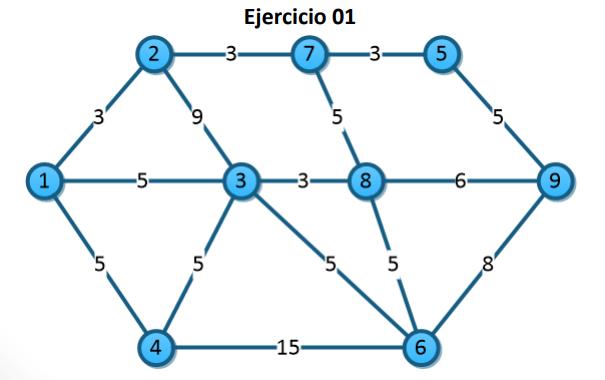
\includegraphics[width=0.8\textwidth]{Abigail/Ejercicio09/Images/1.PNG}
    \end{figure} 

    \subsection{DIJKSTRA}

      \subsubsection{Tabla}
        Ruta más corta desde el nodo 1 hasta los demás.

        En este caso la ruta más costosa es de 14, que va desde el nodo 1 hacia el nodo 9, de igual forma coincide con el camino más largo.

        \begin{figure}[h!]
          \centering
          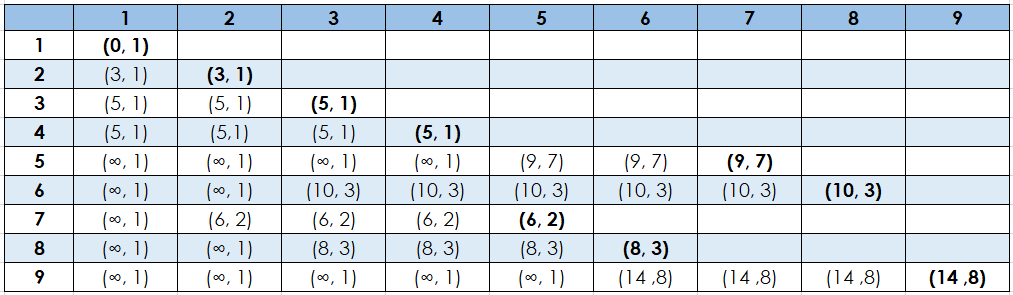
\includegraphics[width=1.1\textwidth]{Abigail/Ejercicio09/Images/1_DT.PNG}
        \end{figure} 
\newpage
      \subsubsection{Resultado}
      
        \begin{figure}[h!]
          \centering
          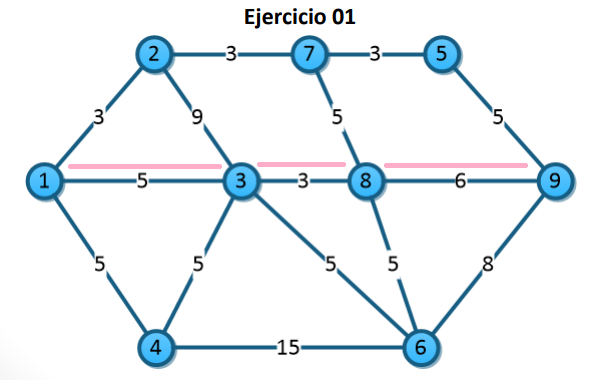
\includegraphics[width=0.7\textwidth]{Abigail/Ejercicio09/Images/1_DR.PNG}
          \caption{Se muestra el camino al último nodo de la tabla}
        \end{figure} 


    \subsection{PRIM}
        \begin{multicols}{2}
            \subsubsection{Tabla}
              
                  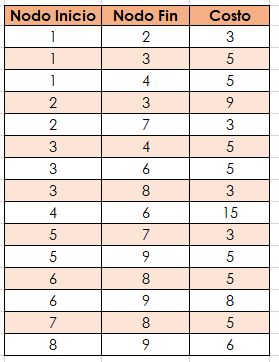
\includegraphics[width=0.4\textwidth]{Abigail/Ejercicio09/Images/1_PT.PNG}
              
        \columnbreak
        
            \subsubsection{Explicación}
                \begin{itemize}
        
                  \item[\checkmark] Crear tabla de las aristas junto a sus costos.
        
                  \item[\checkmark] Nos colocamos en el nodo $1$ y buscamos quién tiene el menor costo, en este caso hacia el nodo $2$ tiene costo $3$.
                  
                  \item[\checkmark] Nos colocamos en el nodo $2$, vemos hacia que nodos podemos llegar y no han sido tocados, comparamos sus costos, en este caso ir al nodo $7$ desde el nodo $2$ es menos costoso.
         
                  \item[\checkmark] Hacemos lo mismo para los demás nodos, siempre comparando y eligiendo al que tiene menor costo en los nodos que no hemos pasado.
        
                \end{itemize}
        \end{multicols}
\newpage

      \subsubsection{Resultado}
        \begin{figure}[h!]
          \centering
          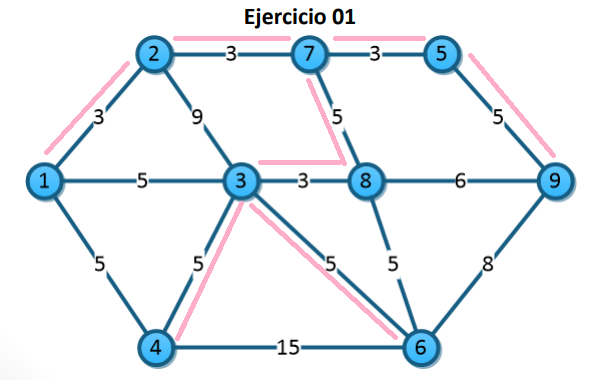
\includegraphics[width=0.7\textwidth]{Abigail/Ejercicio09/Images/1_PR.PNG}
           \caption{Resultado del recorrido que tiene menos costo, siendo este: 32}
        \end{figure} 

    \subsection{KRUSKAL}
        \begin{multicols}{2}
            \subsubsection{Tabla}
              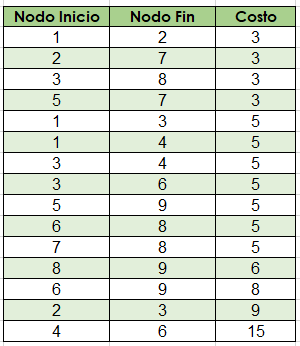
\includegraphics[width=0.5\textwidth]{Abigail/Ejercicio09/Images/1_KT.PNG}
              
        \columnbreak
        
            \subsubsection{Explicación}
                \begin{itemize}
        
                 \item[\checkmark] Crear tabla de las aristas junto a sus costos pero ordenados de menor a mayor costo.

                  \item[\checkmark] Nos colocamos en el nodo $1$ y agarramos al siguiente elemento en la tabla, en este caso el nodo $2$.
                  
                  \item[\checkmark] La tabla nos indica que nos coloquemos en el nodo $2$ y conectemos al nodo $7$.
                  
                  \item[\checkmark] Hacemos lo mismo para los demás nodos, cuidando de no caer en un ciclo, como sucede en el caso del nodo $3$ al $4$.
        
                \end{itemize}
        \end{multicols}
    \newpage
      \subsubsection{Resultado}

        \begin{figure}[h!]
          \centering
            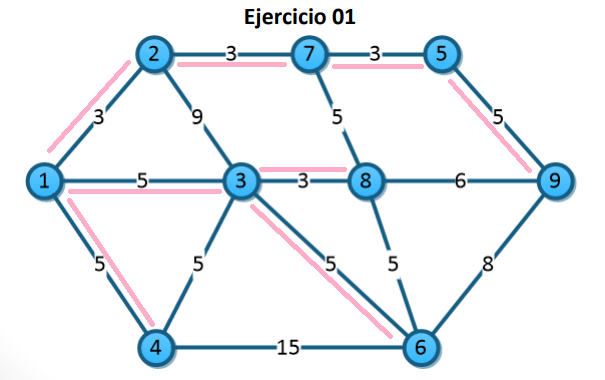
\includegraphics[width=0.8\textwidth]{Abigail/Ejercicio09/Images/1_KR.PNG}
            \caption{Resultado del recorrido que tiene menos costo, siendo este: 32}
        \end{figure} 

  % -----------------------------------------------
  %                   EJERCICIO 02
  % -----------------------------------------------
  
  \section{Ejercicio 02}

    \begin{figure}[h!]
      \centering
      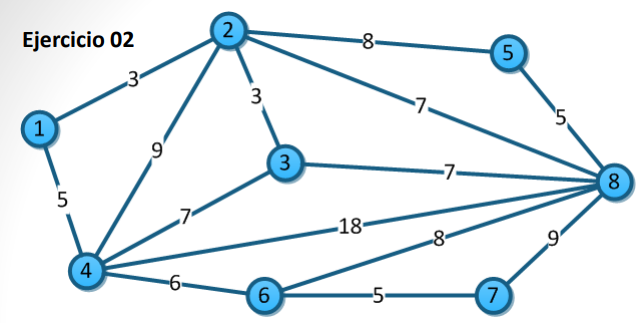
\includegraphics[width=0.9\textwidth]{Abigail/Ejercicio09/Images/2.PNG}
    \end{figure} 

    \subsection{DIJKSTRA}

      \subsubsection{Tabla}
        Ruta más corta desde el nodo 1 hasta los demás.
        
        En este caso la ruta más costosa es de 16 , que va desde el nodo 1 hacia el nodo 7.
        
        \begin{figure}[h!]
          \centering
          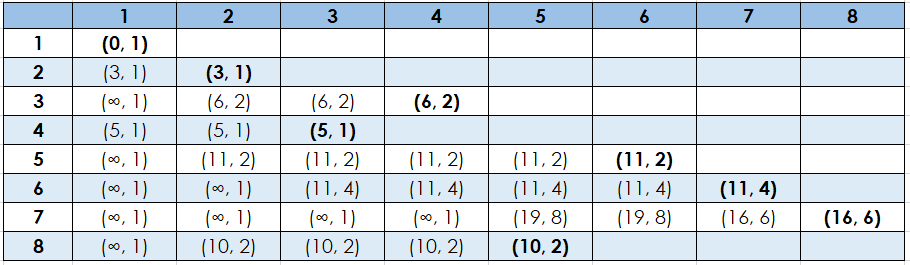
\includegraphics[width=1.1\textwidth]{Abigail/Ejercicio09/Images/2_DT.PNG}
        \end{figure} 

      \subsubsection{Resultado}
        \begin{figure}[h!]
          \centering
          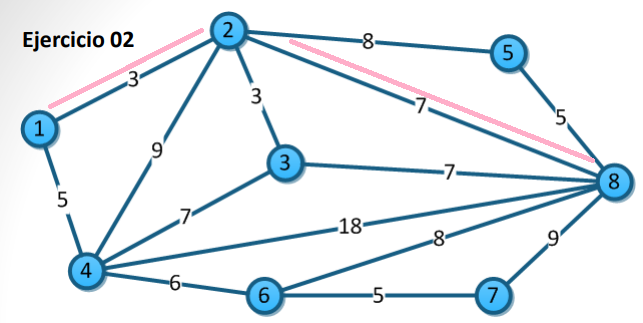
\includegraphics[width=0.9\textwidth]{Abigail/Ejercicio09/Images/2_DR.PNG}
          \caption{Se muestra el último nodo de la tabla}
        \end{figure} 

 \newpage
    \subsection{PRIM}
    \begin{multicols}{2}
            \subsubsection{Tabla}
                  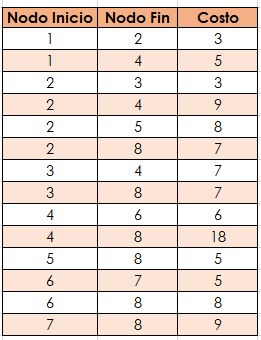
\includegraphics[width=0.4\textwidth]{Abigail/Ejercicio09/Images/2_PT.PNG}
              
        \columnbreak
        
            \subsubsection{Explicación}
                \begin{itemize}
        
                  \item[\checkmark] Crear tabla de las aristas junto a sus costos.
        
                  \item[\checkmark] Nos colocamos en el nodo $1$ y buscamos quién tiene el menor costo, en este caso hacia el nodo $2$ tiene costo $3$.
                  
                  \item[\checkmark] Nos colocamos en el nodo $2$, vemos hacia que nodos podemos llegar y no han sido tocados, comparamos sus costos, en este caso ir al nodo $4$ desde el nodo $2$ es menos costoso.
         
                  \item[\checkmark] Hacemos lo mismo para los demás nodos, siempre comparando y eligiendo al que tiene menor costo en los nodos que no hemos pasado.
        
                \end{itemize}
        \end{multicols}

      \subsubsection{Resultado}
        \begin{figure}[h!]
          \centering
          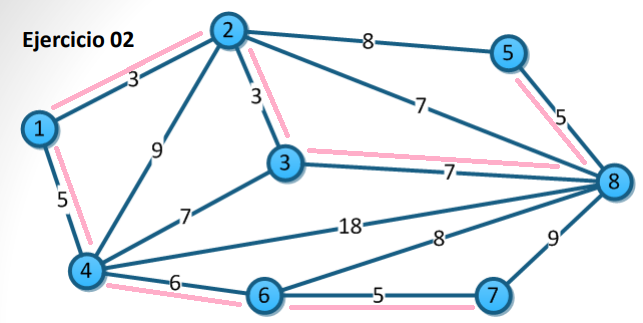
\includegraphics[width=0.8\textwidth]{Abigail/Ejercicio09/Images/2_PR.PNG}
          \caption{Resultado del recorrido que tiene menos costo, siendo este: 34}
        \end{figure} 
\newpage
    
    \subsection{KRUSKAL}
        \begin{multicols}{2}
                \subsubsection{Tabla}
                 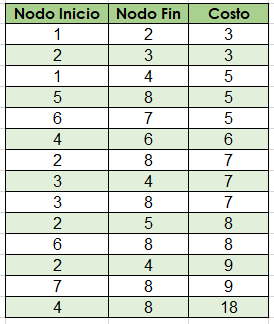
\includegraphics[width=0.4\textwidth]{Abigail/Ejercicio09/Images/2_KT.PNG}
                  
            \columnbreak
            
                \subsubsection{Explicación}
                    \begin{itemize}
            
                     \item[\checkmark] Crear tabla de las aristas junto a sus costos pero ordenados de menor a mayor costo.
    
                      \item[\checkmark] Nos colocamos en el nodo $1$ y agarramos al siguiente elemento en la tabla, en este caso el nodo $2$.
                      
                      \item[\checkmark] La tabla nos indica que nos coloquemos en el nodo $2$ y conectemos al nodo $3$.
                      
                      \item[\checkmark] Hacemos lo mismo para los demás nodos, cuidando de no caer en un ciclo, como sucede en el caso del nodo $3$ al $4$.
            
                    \end{itemize}
            \end{multicols}

      \subsubsection{Resultado}

        \begin{figure}[h!]
          \centering
          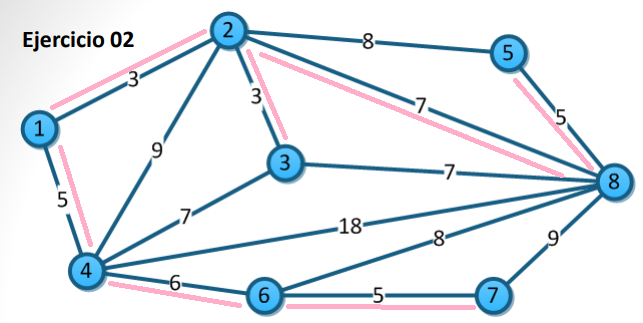
\includegraphics[width=0.8\textwidth]{Abigail/Ejercicio09/Images/2_KR.PNG}
          \caption{Resultado del recorrido que tiene menos costo, siendo este: 34}
        \end{figure} 
\newpage
  % -----------------------------------------------
  %                   EJERCICIO 03
  % -----------------------------------------------
  
  \section{Ejercicio 03}
    \begin{figure}[h!]
      \centering
      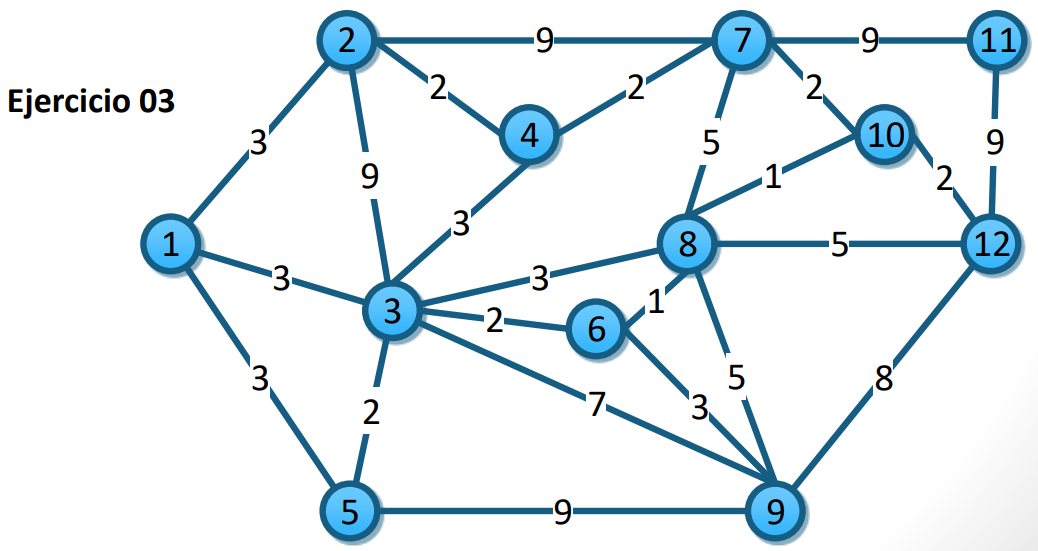
\includegraphics[width=0.9\textwidth]{Abigail/Ejercicio09/Images/3.PNG}
    \end{figure} 

    \subsection{DIJKSTRA}
      \subsubsection{Tabla}
        Ruta más corta desde el nodo 1 hasta los demás.
        
        En este caso la ruta más costosa es de 16 , que va desde el nodo 1 hacia el nodo 7.
      
        \begin{figure}[h!]
          \centering
          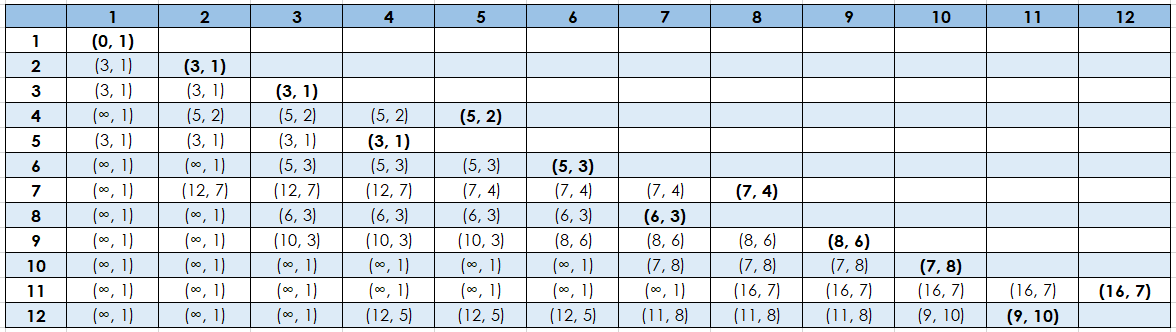
\includegraphics[width=1.1\textwidth]{Abigail/Ejercicio09/Images/3_DT.PNG}
          
        \end{figure} 
\newpage
      \subsubsection{Resultado}
        \begin{figure}[h!]
          \centering
          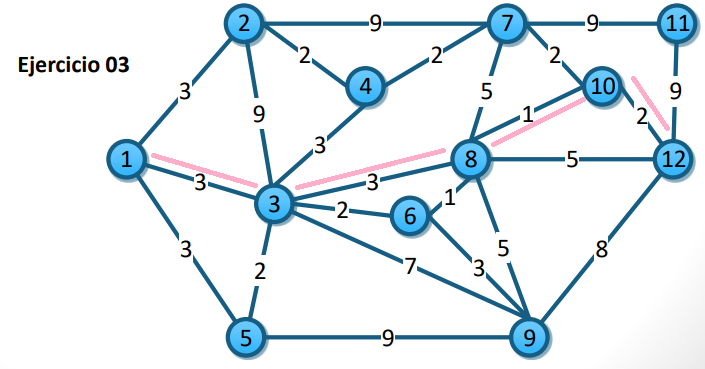
\includegraphics[width=0.9\textwidth]{Abigail/Ejercicio09/Images/3_DR.PNG}
          \caption{Se muestra el último nodo de la tabla}
        \end{figure} 

    \subsection{PRIM}

      \subsubsection{Tabla}

        \begin{figure}[h!]
          \centering
          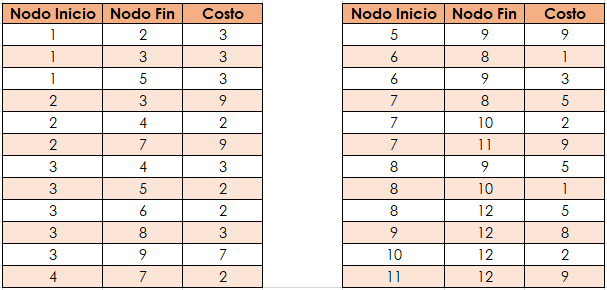
\includegraphics[width=1.0\textwidth]{Abigail/Ejercicio09/Images/3_PT.PNG}
        \end{figure} 
        
         \subsubsection{Explicación}
            \begin{itemize}
    
              \item[\checkmark] Crear tabla de las aristas junto a sus costos.
    
              \item[\checkmark] Nos colocamos en el nodo $1$ y buscamos quién tiene el menor costo, en este caso hacia el nodo $2$ tiene costo $3$.
              
              \item[\checkmark] Nos colocamos en el nodo $2$, vemos hacia que nodos podemos llegar y no han sido tocados, comparamos sus costos, en este caso ir al nodo $4$ desde el nodo $2$ es menos costoso.
            
              \item[\checkmark] Nos colocamos en el nodo $4$, vemos hacia que nodos podemos llegar y no han sido tocados, comparamos sus costos, en este caso ir al nodo $7$ desde el nodo $4$ es menos costoso.
              
              \item[\checkmark] Nos colocamos en el nodo $7$, vemos hacia que nodos podemos llegar y no han sido tocados, comparamos sus costos, en este caso ir al nodo $10$ desde el nodo $7$ es menos costoso.
              
               \item[\checkmark] Nos colocamos en el nodo $10$, vemos hacia que nodos podemos llegar y no han sido tocados, comparamos sus costos, en este caso ir al nodo $8$ desde el nodo $10$ es menos costoso.
              
              \item[\checkmark] Hacemos lo mismo para los demás nodos, siempre comparando y eligiendo al que tiene menor costo en los nodos que no hemos pasado.
    
            \end{itemize}
                
      \subsubsection{Resultado}
        \begin{figure}[h!]
          \centering
          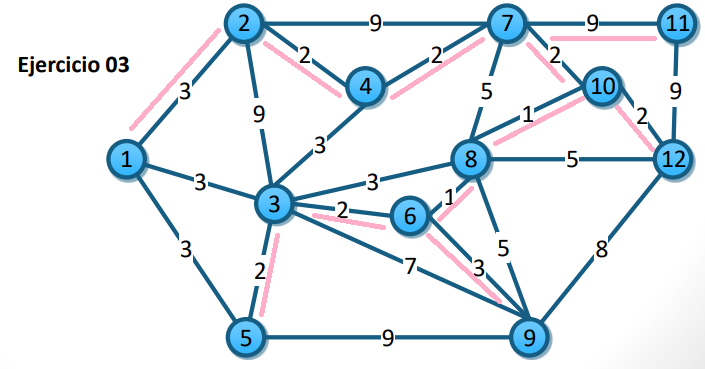
\includegraphics[width=0.8\textwidth]{Abigail/Ejercicio09/Images/3_PR.PNG}
          \caption{Resultado del recorrido que tiene menos costo, siendo este: 29}
        \end{figure} 

\newpage

    \subsection{KRUSKAL}
    
      \subsubsection{Tabla}
        \begin{figure}[h!]
          \centering
          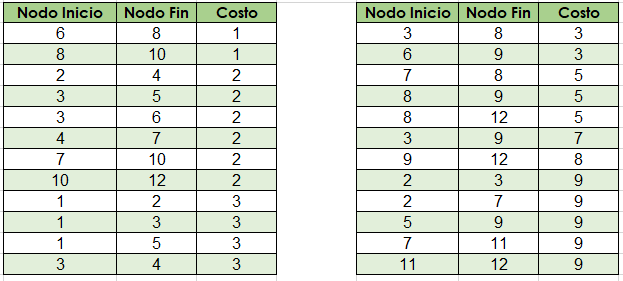
\includegraphics[width=1.0\textwidth]{Abigail/Ejercicio09/Images/3_KT.PNG}
        \end{figure} 
        
        \subsubsection{Explicación}
            \begin{itemize}
    
             \item[\checkmark] Crear tabla de las aristas junto a sus costos pero ordenados de menor a mayor costo.

              \item[\checkmark] Nos colocamos en el nodo $1$ y agarramos al siguiente elemento en la tabla, en este caso el nodo $8$.
              
              \item[\checkmark] La tabla nos indica que nos coloquemos en el nodo $8$ y conectemos al nodo $10$.
              
              \item[\checkmark] La tabla nos indica que nos coloquemos en el nodo $2$ y conectemos al nodo $4$.
              
              \item[\checkmark] La tabla nos indica que nos coloquemos en el nodo $3$ y conectemos al nodo $5$.
              
              \item[\checkmark] La tabla nos indica que nos coloquemos en el nodo $3$ y conectemos al nodo $6$.
              
              \item[\checkmark] La tabla nos indica que nos coloquemos en el nodo $4$ y conectemos al nodo $7$.
              
              \item[\checkmark] La tabla nos indica que nos coloquemos en el nodo $7$ y conectemos al nodo $10$.
              
              \item[\checkmark] La tabla nos indica que nos coloquemos en el nodo $10$ y conectemos al nodo $12$.
              
              \item[\checkmark] La tabla nos indica que nos coloquemos en el nodo $1$ y conectemos al nodo $2$.
              
              \item[\checkmark] Hacemos lo mismo para los demás nodos, cuidando de no caer en un ciclo, como sucede en el caso del nodo $1$ al $3$.
    
            \end{itemize}
\newpage
      \subsubsection{Resultado}

        \begin{figure}[h!]
          \centering
          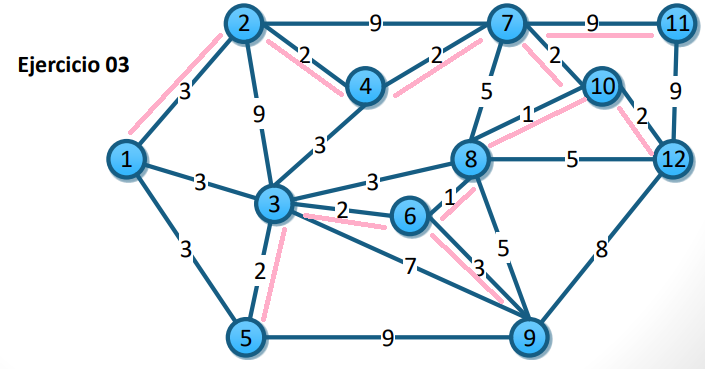
\includegraphics[width=0.9\textwidth]{Abigail/Ejercicio09/Images/3_KR.PNG}
          \caption{Resultado del recorrido que tiene menos costo, siendo este: 29}
        \end{figure} 

  % -----------------------------------------------
  %                   EJERCICIO 04
  % -----------------------------------------------
  
  \section{Ejercicio 04}

    \begin{figure}[h!]
      \centering
      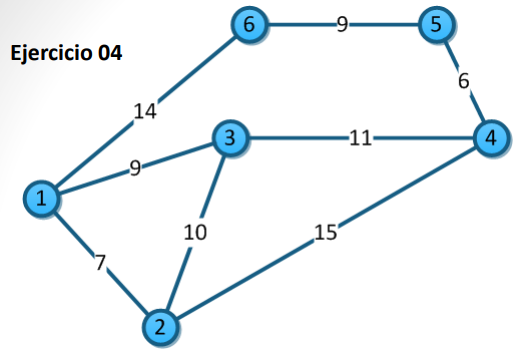
\includegraphics[width=0.8\textwidth]{Abigail/Ejercicio09/Images/4.PNG}
    \end{figure} 

    \subsection{DIJKSTRA}

      \subsubsection{Tabla}
        Ruta más corta desde el nodo 1 hasta los demás.
        
        En este caso la ruta más costosa es de 23 , que va desde el nodo 1 hacia el nodo 5.

        \begin{figure}[h!]
          \centering
          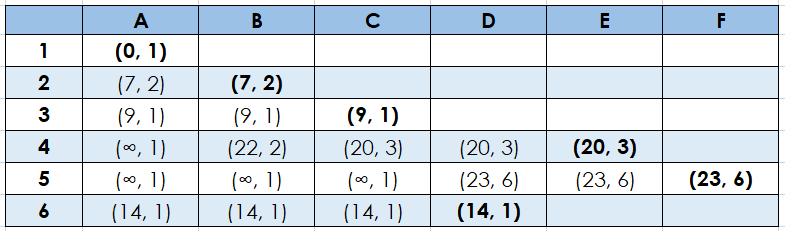
\includegraphics[width=1.0\textwidth]{Abigail/Ejercicio09/Images/4_DT.PNG}
        \end{figure} 

      \subsubsection{Resultado}
        \begin{figure}[h!]
          \centering
          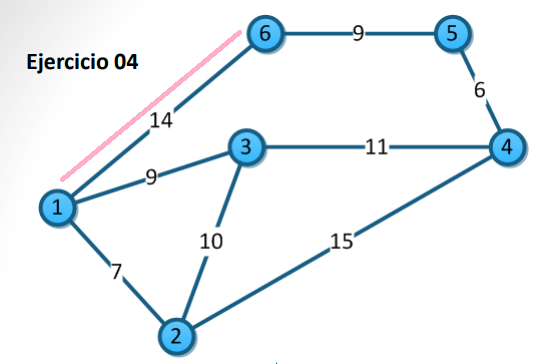
\includegraphics[width=0.8\textwidth]{Abigail/Ejercicio09/Images/4_DR.PNG}
          \caption{Se muestra el último nodo de la tabla}
        \end{figure} 
\newpage
    \subsection{PRIM}
    \begin{multicols}{2}
            \subsubsection{Tabla}
                  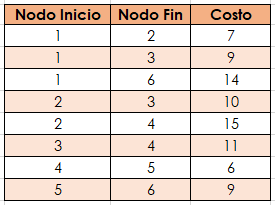
\includegraphics[width=0.4\textwidth]{Abigail/Ejercicio09/Images/4_PT.PNG}
              
        \columnbreak
        
            \subsubsection{Explicación}
                \begin{itemize}
        
                  \item[\checkmark] Crear tabla de las aristas junto a sus costos.
        
                  \item[\checkmark] Nos colocamos en el nodo $1$ y buscamos quién tiene el menor costo, en este caso hacia el nodo $2$ tiene costo $7$.
         
                  \item[\checkmark] Hacemos lo mismo para los demás nodos, siempre comparando y eligiendo al que tiene menor costo en los nodos que no hemos pasado.
        
                \end{itemize}
        \end{multicols}

      \subsubsection{Resultado}
        \begin{figure}[h!]
          \centering
          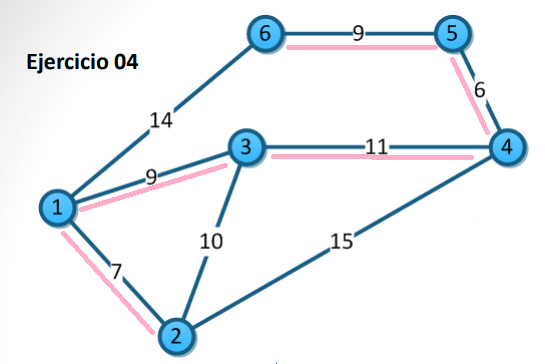
\includegraphics[width=0.8\textwidth]{Abigail/Ejercicio09/Images/4_PR.PNG}
          \caption{Resultado del recorrido que tiene menos costo, siendo este: 42}
        \end{figure} 
\newpage
    \subsection{KRUSKAL}
            \begin{multicols}{2}
                \subsubsection{Tabla}
                 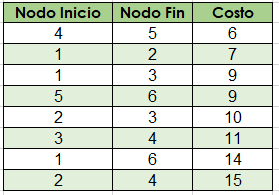
\includegraphics[width=0.4\textwidth]{Abigail/Ejercicio09/Images/4_KT.PNG}
                  
            \columnbreak
            
                \subsubsection{Explicación}
                    \begin{itemize}
            
                     \item[\checkmark] Crear tabla de las aristas junto a sus costos pero ordenados de menor a mayor costo.
    
                      \item[\checkmark] Nos colocamos en el nodo $4$ y agarramos al siguiente elemento en la tabla, en este caso el nodo $5$.
                      
                      \item[\checkmark] Hacemos lo mismo para los demás nodos, cuidando de no caer en un ciclo, como sucede en el caso del nodo $2$ al $3$.
            
                    \end{itemize}
            \end{multicols}

      \subsubsection{Resultado}

        \begin{figure}[h!]
          \centering
          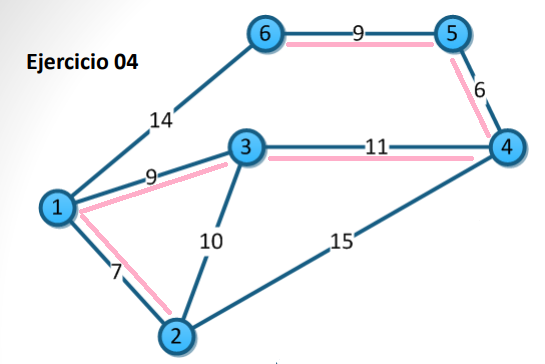
\includegraphics[width=0.8\textwidth]{Abigail/Ejercicio09/Images/4_KR.PNG}
          \caption{Resultado del recorrido que tiene menos costo, siendo este: 42}
        \end{figure} 

\newpage
  % -----------------------------------------------
  %                   EJERCICIO 05
  % -----------------------------------------------
  
  \section{Ejercicio 05}

    \begin{figure}[h!]
      \centering
      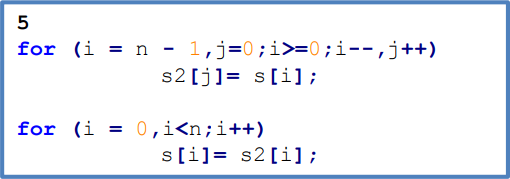
\includegraphics[width=0.8\textwidth]{Abigail/Ejercicio09/Images/5.PNG}
    \end{figure} 

    \subsection{DIJKSTRA}

      \subsubsection{Tabla}
         Ruta más corta desde el nodo 1 hasta los demás.
        
        En este caso la ruta más costosa es de 24 , que va desde el nodo A hacia el nodo Q.

       \begin{figure}[h!]
          \centering
          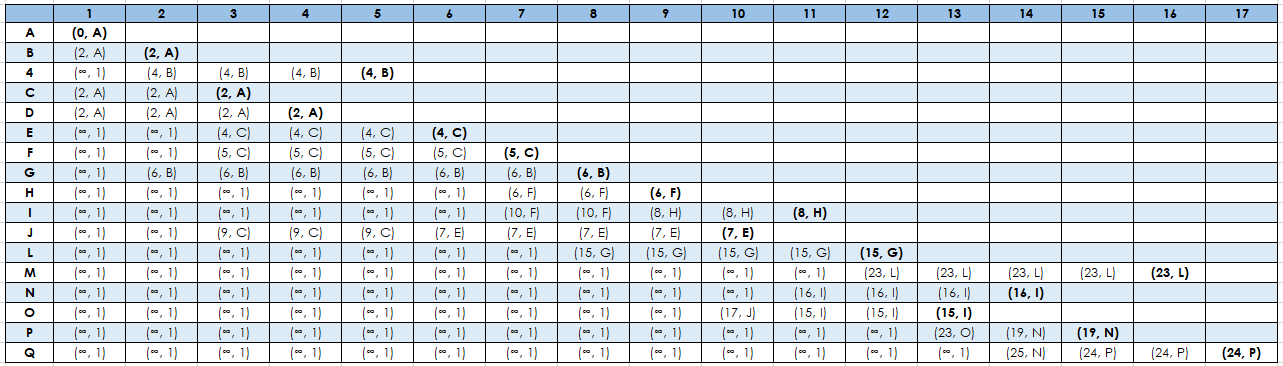
\includegraphics[width=1.1\textwidth]{Abigail/Ejercicio09/Images/5_DT.PNG}
        \end{figure} 
\newpage

      \subsubsection{Resultado}
        \begin{figure}[h!]
          \centering
          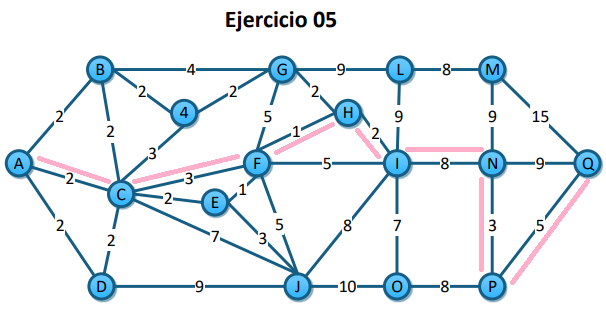
\includegraphics[width=0.8\textwidth]{Abigail/Ejercicio09/Images/5_DR.PNG}
          \caption{Se muestra el último nodo de la tabla}
        \end{figure} 

    \subsection{PRIM}

      \subsubsection{Tabla}
        \begin{figure}[h!]
          \centering
          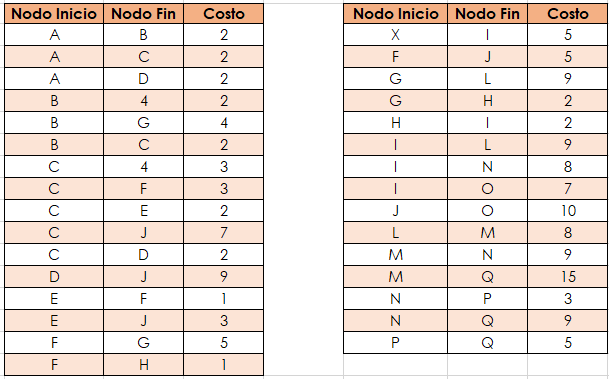
\includegraphics[width=0.8\textwidth]{Abigail/Ejercicio09/Images/5_PT.PNG}
        \end{figure} 

    
        \subsubsection{Explicación}
            \begin{itemize}
    
              \item[\checkmark] Crear tabla de las aristas junto a sus costos.
    
              \item[\checkmark] Nos colocamos en el nodo A y buscamos quién tiene el menor costo, en este caso hacia el nodo B tiene costo $2$.
              
              \item[\checkmark] Nos colocamos en el nodo B, vemos hacia que nodos podemos llegar y no han sido tocados, comparamos sus costos, en este caso ir al nodo $4$ desde el nodo B es menos costoso.
            
              \item[\checkmark] Nos colocamos en el nodo $4$, vemos hacia que nodos podemos llegar y no han sido tocados, comparamos sus costos, en este caso ir al nodo G desde el nodo $4$ es menos costoso.
              
              \item[\checkmark] Nos colocamos en el nodo G, vemos hacia que nodos podemos llegar y no han sido tocados, comparamos sus costos, en este caso ir al nodo C desde el nodo B es menos costoso.
              
               \item[\checkmark] Nos colocamos en el nodo C, vemos hacia que nodos podemos llegar y no han sido tocados, comparamos sus costos, en este caso ir al nodo E desde el nodo C es menos costoso.
              
              \item[\checkmark] Hacemos lo mismo para los demás nodos, siempre comparando y eligiendo al que tiene menor costo en los nodos que no hemos pasado.
    
            \end{itemize}
                
      \subsubsection{Resultado}
        \begin{figure}[h!]
          \centering
          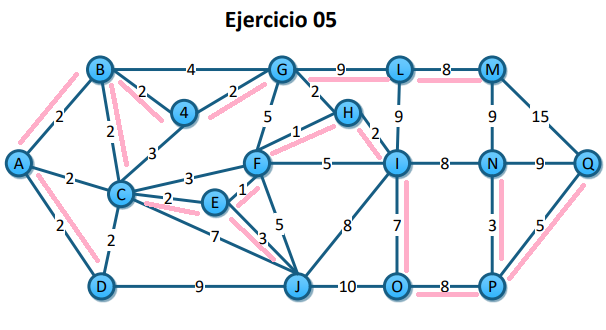
\includegraphics[width=0.8\textwidth]{Abigail/Ejercicio09/Images/5_PR.PNG}
          \caption{Resultado del recorrido que tiene menos costo, siendo este: 59}
        \end{figure} 
    
    \newpage

    \subsection{KRUSKAL}

      \subsubsection{Tabla}
        \begin{figure}[h!]
          \centering
          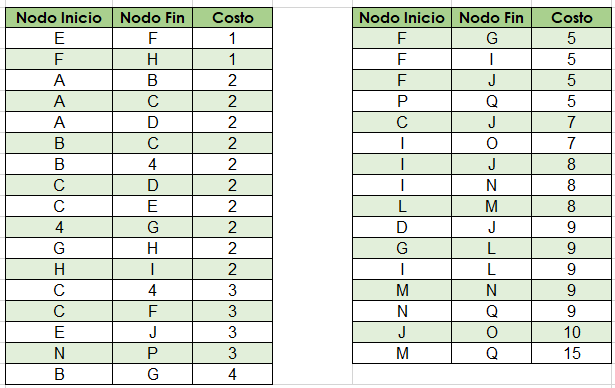
\includegraphics[width=0.8\textwidth]{Abigail/Ejercicio09/Images/5_KT.PNG}
        \end{figure} 
        
        \subsubsection{Explicación}
            \begin{itemize}
    
             \item[\checkmark] Crear tabla de las aristas junto a sus costos pero ordenados de menor a mayor costo.

              \item[\checkmark] Nos colocamos en el nodo E y agarramos al siguiente elemento en la tabla, en este caso el nodo F.
              
              \item[\checkmark] La tabla nos indica que nos coloquemos en el nodo F y conectemos al nodo H.
              
              \item[\checkmark] La tabla nos indica que nos coloquemos en el nodo A y conectemos al nodo B.
              
              \item[\checkmark] La tabla nos indica que nos coloquemos en el nodo A y conectemos al nodo C.
              
              \item[\checkmark] La tabla nos indica que nos coloquemos en el nodo A y conectemos al nodo D.
              
              \item[\checkmark] La tabla nos indica que nos coloquemos en el nodo B y conectemos al nodo $4$.
              
              \item[\checkmark] Hacemos lo mismo para los demás nodos, cuidando de no caer en un ciclo, como sucede en el caso del nodo B al C.
    
            \end{itemize}
\newpage
      \subsubsection{Resultado}

        \begin{figure}[h!]
          \centering
          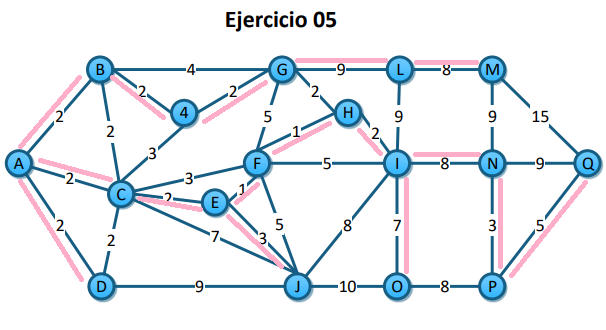
\includegraphics[width=0.7\textwidth]{Abigail/Ejercicio09/Images/5_KR.PNG}
          \caption{Resultado del recorrido que tiene menos costo, siendo este: 59}
        \end{figure} 
\end{document}